\documentclass[12pt]{article}

\usepackage[utf8]{inputenc}


\usepackage{caption}
\usepackage{amsmath}
\usepackage{graphicx}
\usepackage{amssymb}
\usepackage{float}
\usepackage{multirow}
\usepackage{setspace} \setstretch{0.9}
% set font size to 11pt


\setlength{\parskip}{\baselineskip}%
\setlength{\parindent}{0pt}%


\begin{document}

\title{Spectrum Analysis}
\author{lwp26}
\date{Feburary 2023}
\maketitle

\begin{abstract}
    \centering
    This report will discuss the use of spectrum analysis in the study of signals by looking at the spectrum of various waveforms and the spectrum of amplitude modulated signals. The report will also discuss the use of a simple demodulator to recover the original signal from the amplitude modulated signal.
\end{abstract}


\section{Introduction}

\subsection{Background}
Spectral analysis is important in signal processing because it allows the frequency content of a signal to be analyzed, which is useful for identifying the physical properties of the signal source. Spectral analysis is used in many areas of science and engineering, such as acoustics, communications, medical imaging, and astronomy, for tasks such as noise reduction, signal filtering, feature extraction, pattern recognition, and data compression.

Amplitude modulation (AM) is a technique used in telecommunications and broadcasting to transmit information by varying the amplitude of a carrier wave. AM is widely used in radio broadcasting, where it allows multiple stations to share the same frequency band and transmit information to a large audience.

\subsection{Aims}

\begin{itemize}
    \item To introduce the concept of spectrum analysis
    \item To become aquainted with the use of simple computer based spectrum analyser software.
    \item To measure the spectra of various simple waveforms.
    \item To study the spectra of amplitude modulated signals and characteristics of a simple demodulator.
\end{itemize}

\section{Method and Theory}

\subsection{Measuring the Spectrum of Signals}

Square and triangle waves can be split into a series of sine and cosine waves at discrete frequencies. The Fourier series of a signal is given by

\begin{equation}
    x(t) = a_0 + \sum_{n=1}^{\infty} a_n \sin(2\pi n f_0 t) + b_n \cos(2\pi n f_0 t)
    \label{eq:1}
\end{equation}

From equation \ref{eq:1} it can see that the Fourier series of a signal is the sum of a constant term, a series of sine terms and a series of cosine terms. 
The terms $a_n$ and $b_n$ are the Fourier coefficients of the signal and signal power at the $n^{th}$ harmonic is given by $P_n = a_n^2 + b_n^2$.

Square wave fourier series
\begin{equation}
    f(t) = \frac{4}{\pi} \sum_{\text{odd n}}^{\infty} \frac{1}{n} \sin\left(n \omega_0 t\right)
    \label{eq:2}
\end{equation}

Triangle wave fourier series
\begin{equation}
    f(t) = \frac{8}{\pi^2} \sum_{\text{odd n}}^{\infty} \pm \frac{1}{n^2} \sin\left(n\omega_0 t\right)
    \label{eq:3}
\end{equation}
where signs alternate, $+$ for $n = 1$

From this it can be seen that the frequency components of the signal decay as $1/n^2$ for the triangle wave and $1/n$ for the square wave. This means that the higher harmonics of the signal have a much smaller amplitude than the lower harmonics.

\subsection{Amplitude Modulation}

Considering a simple information signal $x(t) = E cos(\omega t)$ and a carrier signal $x_c(t) = E_c cos(\omega_0 t)$, the amplitude modulated signal is generated by multiplying the carrier signal with the offsetted information signal as shown below
\begin{equation}
    x_m(t) = E_c(1+m cos(\omega_ct))cos(\omega_0t)
    \label{eq:4}
\end{equation}

Expanding the above gives

\begin{equation}
    x_m(t) = E_c cos(\omega_c t) + \frac{m E_c}{2}cos((\omega_c + \omega_0)t) + \frac{m E_c}{2}cos((\omega_c - \omega_0)t)
    \label{eq:5}
\end{equation}

This shows that the modulated signal has three frequency components, the carrier frequency, the carrier frequency plus the information frequency and the carrier frequency minus the information frequency. The amplitude of the information frequency components is given by $mE_c/2$.

The modulation index can be measured on the frequency spectrum by $m = \frac{2E_c}{E_{fc}} $ where $E_c$ is the frequency component at the carrier frequency and $E_{fc}$ is the frequency component at the carrier frequency plus the information frequency.
The modulation index can also be measured by finding the ratio of maximum and minimum values of the envelope of the modulated signal using eq \ref{eq:6} seen below.
\begin{equation}
    \frac{1+m}{1-m} = \frac{V_{e,max}}{V_{e,min}}
    \label{eq:6}
\end{equation}

\subsection{Amplitude Demodulation}

\begin{figure}[h]
    \centering
    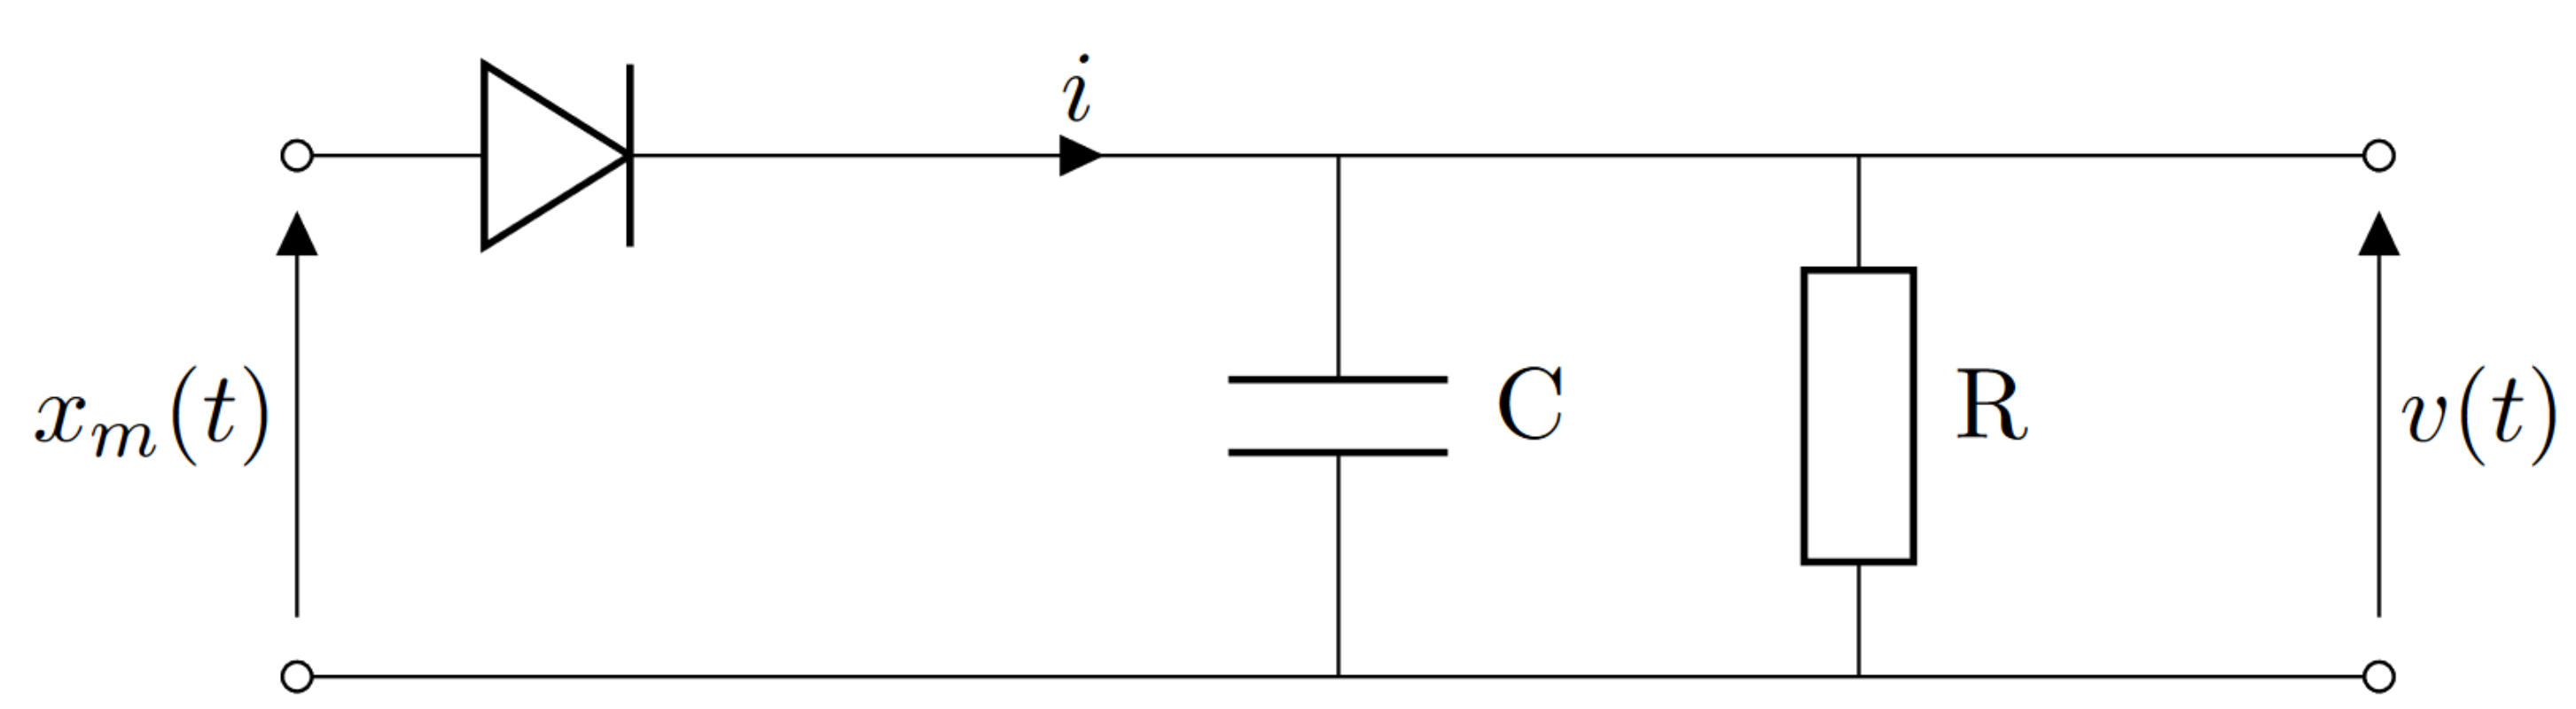
\includegraphics[width=0.8\textwidth]{demod_circuit.png}
    \caption{Demodulator circuit diagram}
    \label{fig:demod_circuit}
\end{figure}

In this circuit the step down response from $v_0$ is derived and given as

\begin{equation}
    v(t) = v_0 e^{-\frac{t}{RC}}
    \label{eq:7}
\end{equation}

When we connect a time varying input, $x_m(t)$ the capacitor will alternate
between charging and discharging cycles. During the charging cycle, the capacitor's voltage $v(t)$ will
track the input or $v(t) = xm(t)$. During the discharging cycle, $v(t)$ will decay like Equation \ref{eq:4}. Discharge
will persist until $x_m(t)$ rises to match the falling value of v(t), when the circuit switches to charging.
Charging will end when xm(t) begins to fall again.

Therefor the output of the circuit can be given by

\begin{equation}
    v(t) = 
    \begin{cases}
        v(\tau)e^{-\frac{1}{RC}(t-\tau)}, & \text{if} \ x_m(t) < v(\tau)e^{-\frac{1}{RC}(t-\tau)} \\
        x_m(t), & \text{otherwise}
    \end{cases}
    \label{eq:8}
\end{equation}

\subsection{Apparatus and Setup}

\begin{figure}[h]
    \centering
    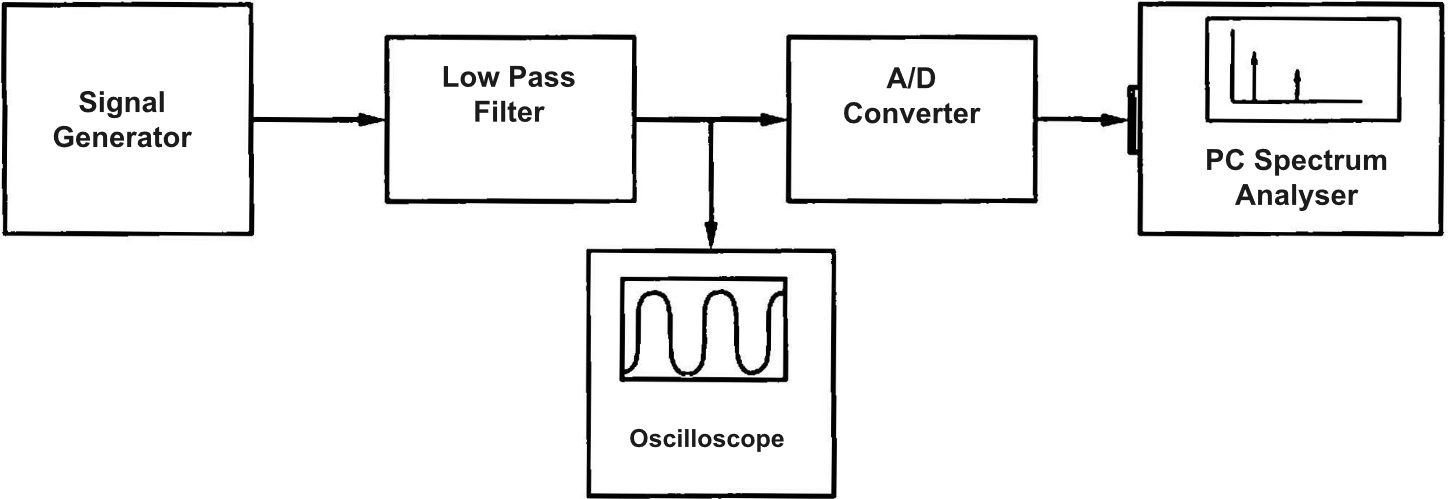
\includegraphics[width=0.8\textwidth]{setup_diagram.png}
    \caption{Graph showing block diagram setup}
    \label{fig:setup}
\end{figure}

This experiment was carried out using a PicoScope as a spectrum analyser using the PicoScope 6 software. The PicoScope was connected to a computer via USB and the PicoScope 6 software was used to display the linear spectrum of the signals.
The signal generator used a chip made by Analog Devices to make precise waveforms.

% add about how the low pass filter or anti aliasing filter was set up, 2khz low pass filter
% add about how the picoscope was set up linear 


\section{Results}

\begin{table}[h]
    \centering
    \caption{Frequency composition for Triangle Wave}
    \begin{tabular}{|c|c|}
    \hline
    Frequency (kHz) & Voltage (mV) \\ \hline
    0.998           & 546.4        \\
    2.992           & 62.9         \\
    4.986           & 22.28        \\
    6.98            & 10.88        \\
    8.987           & 4.895        \\ \hline
    \end{tabular}
\end{table}

\begin{table}[h]
    \centering
    \caption{Frequency composition for Square Wave}
    \begin{tabular}{|c|c|}
    \hline
    Frequency (kHz) & Voltage (mV) \\ \hline
    0.998           & 846.1        \\
    2.998           & 258          \\
    4.995           & 159.6        \\
    6.992           & 98.89        \\
    8.991           & 73.18        \\ \hline
    \end{tabular}
\end{table}

\begin{figure}[h]
    \centering
    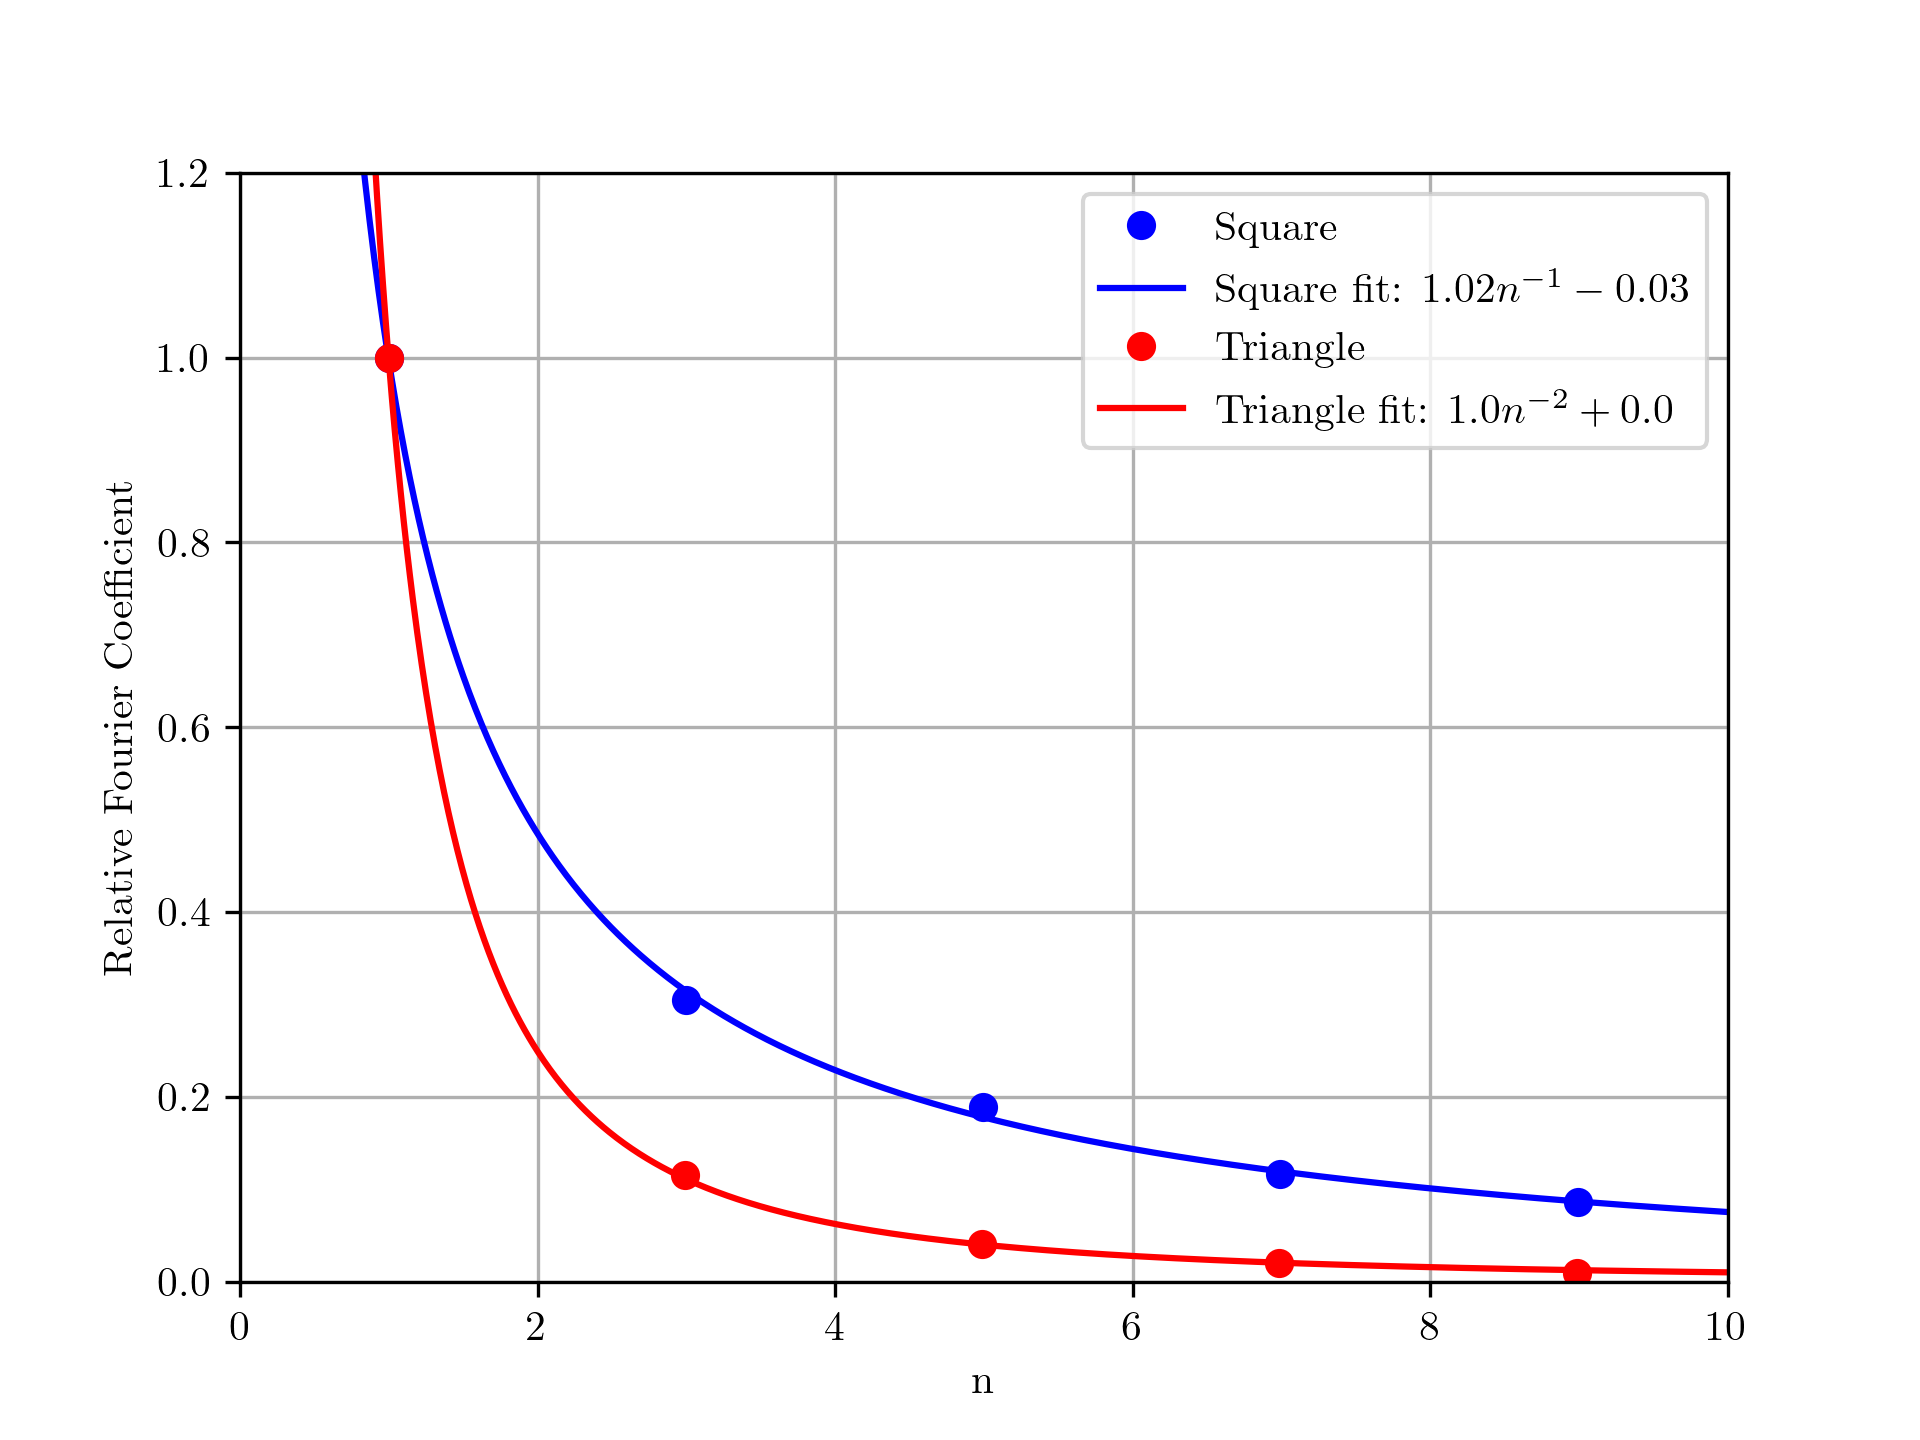
\includegraphics[width=1\textwidth]{square_triangle.png}
    \caption{Graph showing measured square and triangle frequency components and predicted fit}
    \label{fig:square_triangle}
\end{figure}

\begin{figure}[h]
    \centering
    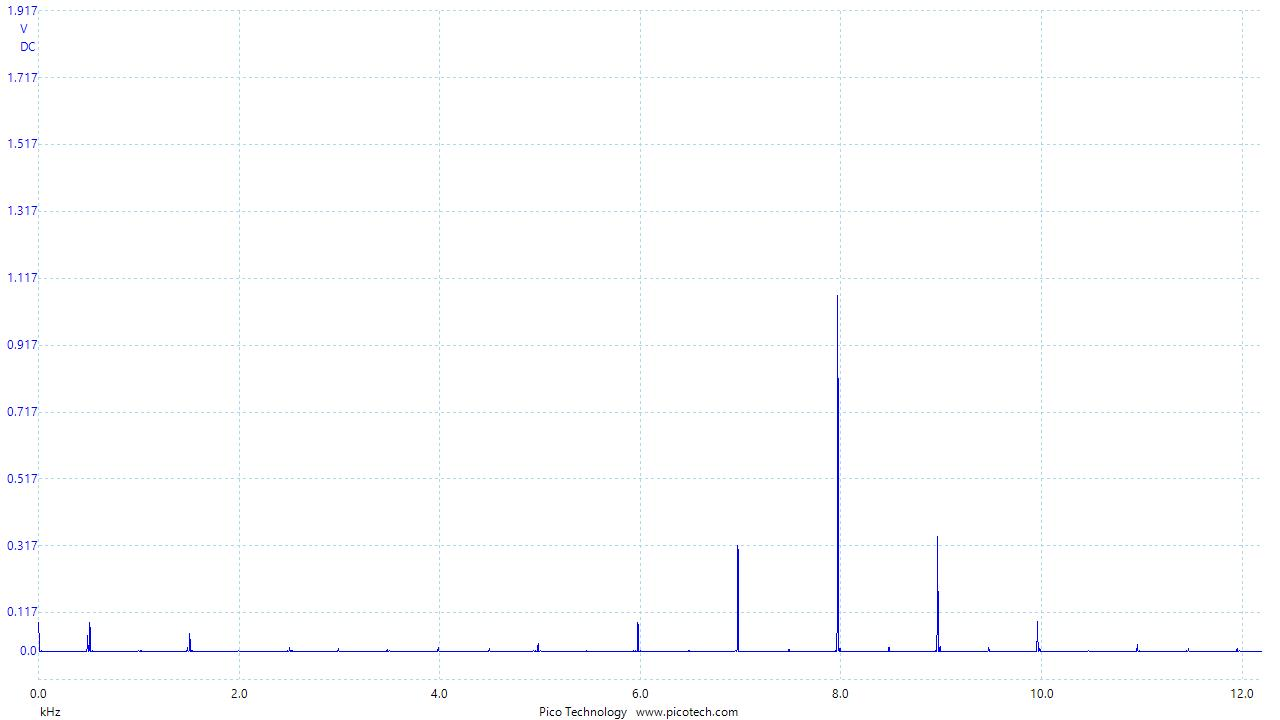
\includegraphics[width=0.8\textwidth]{AmpMod_f.jpg}
    \caption{Graph showing spectrum of amplitude modulated signal}
    \label{fig:freq_responses}
\end{figure}

For the modulated signal, the carrier frequency was set to $7969$ Hz (8KHz) 



\section{Analysis of results}




\section{Conclusion}


\end{document}